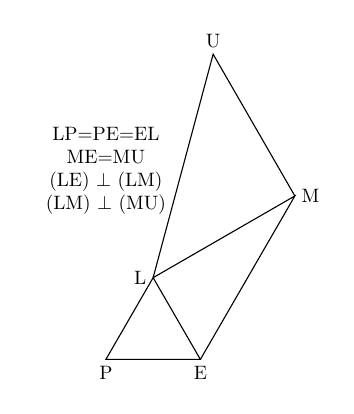
\begin{tikzpicture}[scale=0.6,every node/.style={scale=0.7},rotate=0]

\draw (0,0) node [below]{P}--(2,0) node[below] {E}--(1,1.73) node[left] {L}--cycle;
\draw (1,1.73)--(4,3.46) node[right] {M}--(2,0);
\draw (1,1.73)--(2.27,6.46) node[above] {U}--(4,3.46);
\node at(0,4) {\begin{tabular}{c} LP=PE=EL \\ ME=MU \\ (LE) $\perp$ (LM) \\(LM) $\perp$ (MU)  \end{tabular}};

\end{tikzpicture}